% !TeX program = pdflatex
\documentclass[border=6pt]{standalone}
\usepackage{tikz}
\usetikzlibrary{arrows.meta, positioning, shapes.geometric, backgrounds}

% ---- Paleta del tema SimpleDarkBlue ----
\definecolor{MediumRed}{rgb}{0.925, 0.345, 0.345}
\definecolor{MediumGreen}{rgb}{0.37, 0.7, 0.66}
\definecolor{MediumBlue}{rgb}{0.015, 0.315, 0.45}
\definecolor{DarkBlue}{rgb}{0.05, 0.15, 0.35}

\begin{document}
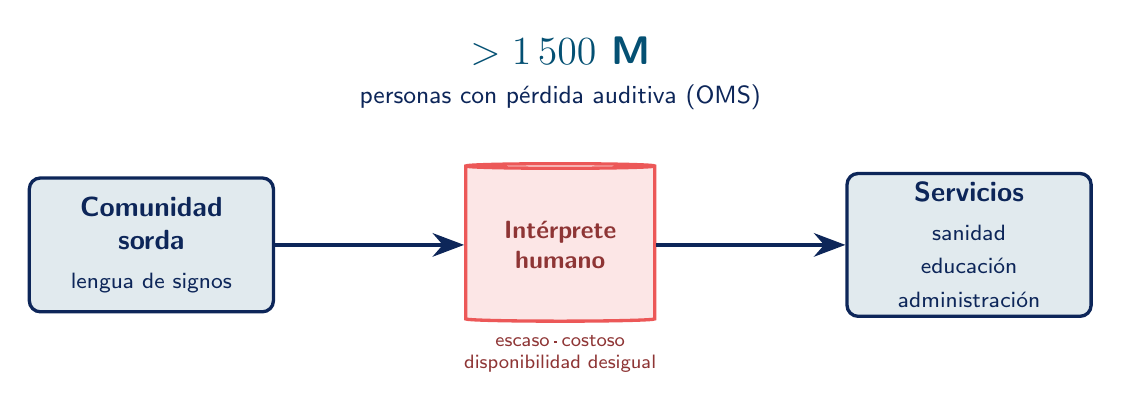
\begin{tikzpicture}[
    font=\sffamily,
    endpoint/.style={draw=DarkBlue, very thick, rounded corners=4pt,
        fill=MediumBlue!12, minimum width=3.1cm, minimum height=1.7cm,
        align=center, text=DarkBlue},
    bottleneck/.style={draw=MediumRed, very thick, fill=MediumRed!15,
        align=center, text=MediumRed!60!black,
        cylinder, shape border rotate=90, aspect=0.25,
        minimum width=2.4cm, minimum height=2.0cm},
    flow/.style={-{Stealth[length=4mm]}, line width=1.2pt, DarkBlue},
]

% nodos principales
\node[endpoint] (deaf) {\textbf{Comunidad}\\\textbf{sorda}\\[2pt]\footnotesize lengua de signos};
\node[bottleneck, right=2.4cm of deaf] (interp) {};
\node[endpoint, right=2.4cm of interp] (serv)
    {\textbf{Servicios}\\[2pt]\footnotesize sanidad\\\footnotesize educación\\\footnotesize administración};

% etiqueta del cuello de botella
\node[align=center, text=MediumRed!60!black, font=\sffamily\small] at (interp.center)
    {\textbf{Intérprete}\\\textbf{humano}};
\node[align=center, font=\sffamily\scriptsize, text=MediumRed!60!black,
      below=1pt of interp] {escaso\,·\,costoso\\disponibilidad desigual};

% flujos
\draw[flow] (deaf) -- (interp);
\draw[flow] (interp) -- (serv);

% cifras OMS arriba
\node[font=\sffamily\bfseries\Large, text=MediumBlue, above=1.1cm of interp] (n1)
    {$>1\,500$ M};
\node[font=\sffamily\small, text=DarkBlue, below=0pt of n1]
    {personas con pérdida auditiva (OMS)};

\end{tikzpicture}
\end{document}
